\documentclass{beamer}
\usepackage[english]{babel}
\usepackage{biblatex}
\usepackage{tikz}
\usepackage{color}
\usepackage{listings}
\usepackage{amsmath}

\lstset{frame=tb,
  aboveskip=3mm,
  belowskip=3mm,
  showstringspaces=false,
  columns=flexible,
  basicstyle={\small\ttfamily},
  numbers=none,
  numberstyle=\tiny\color{gray},
  keywordstyle=\color{blue},
  commentstyle=\color{dkgreen},
  stringstyle=\color{mauve},
  breaklines=false,
  breakatwhitespace=true,
  tabsize=4
}

\def\R{\mathbb{R}}
\newcommand{\p}{ }

\newtheorem{gs}{General Solution}

\newcommand{\cb}{\color{blue}}
\newcommand{\cred}{\color{red}}
\newcommand{\cg}{\color{green}}
\newcommand{\cbr}{\color{Brown}}
\newcommand{\cm}{\color{Magenta}}
%\newcommand{\cb}{\color{blue}}
\newcommand{\dsp}{\displaystyle}

\newcommand{\fby}{\fcolorbox{blue}{yellow}}
\newcommand{\fbw}{\fcolorbox{blue}{white}}
\def \stackt{{\stackrel{.}{.\;.}\;\;}}
\def \stackb{{\stackrel{.\;.}{.}\;\;}}

\def\diam{\mathrm{diam}\,}
\def\p{\partial}
\def\O{\Omega}
\def\R{\mathbb{R}}
\def\cE{\mathcal{E}}
\def\cT{\mathcal{T}}
\def\cB{\mathcal{B}}
\def\cA{\mathcal{A}}
\def\cN{\mathcal{N}}
\def\Sides{\mathcal{E}_h}
\def\Jump#1{\Big[\!\!\Big[#1\Big]\!\!\Big]}
\def\mJump#1{\big[\hskip -3pt\big[#1\big]\hskip -3pt\big]}
\def\jump#1{[\![#1]\!]}
\def\Mean#1{\Big\{\!\!\!\Big\{#1\Big\}\!\!\!\Big\}}
\def\mMean#1{\big\{\hskip -4pt\big\{#1\big\}\hskip -4pt\big\}}
\def\mean#1{\{\!\!\{#1\}\!\!\}}
\def\cT{\mathcal{T}}
\def\cE{\mathcal{E}}
\def\ssT{{\scriptscriptstyle T}}
\def\sjump#1{[\hskip -1.5pt[#1]\hskip -1.5pt]}
\def\d{\displaystyle}
\newcommand\Blesssim{\;\raise 2pt\hbox{$<$}\hskip -16pt
  \lower 9pt\hbox{$\sim$}\;}
  \newcommand{\pa}{\partial}
  \newcommand{\del}{\bigtriangleup}
%\newcommand\lesssim{\;\raise 2pt\hbox{$<$}\hskip -14pt
%  \lower 8pt\hbox{$\sim$}\;}
\newcommand\alesssim{\raise 2pt\hbox{$<$}\hskip -14pt
  \lower 8pt\hbox{$\sim$}\;}
\def\deq{\,\raise 4pt\hbox{\tiny def}\hskip -10pt\lower
 4pt\hbox{$=$}\;}
\def\tbar{|\!|\!|}
\def\therefore{\hbox{\bf .}\hskip 2pt\hbox{\bf .}
 \hskip -12.5pt\raise 6pt\hbox{\bf .}\hskip 16pt}
\def\so{{\scriptscriptstyle 1}}
\def\st{{\scriptscriptstyle 2}}
\def\sth{{\scriptscriptstyle 3}}
\def\sz{{\scriptscriptstyle 0}}
\def\tR{{R'}}
\def\sf{{\scriptscriptstyle 4}}
\def\bE{\mathbb{E}}
\def\bA{\mathbb{A}}
%
\def\bu{\boldsymbol{u}}
\def\ba{\boldsymbol{a}}
\def\bsi{\boldsymbol{\sigma}}
\def\btau{\boldsymbol{\tau}}
\def\buz{\mathaccent'27{\bu}}
\def\bzz{\mathaccent'27{\bz}}
\def\bq{\boldsymbol{q}}
\def\bw{\boldsymbol{w}}
\def\bW{\boldsymbol{W}}
\def\bz{\boldsymbol{z}}
\def\bn{\boldsymbol{n}}
\def\bof{\boldsymbol{f}}
\def\curl{\nabla\times}
\def\div{\nabla\cdot}
\def\curlh{\nabla_h\times}
\def\ncross{{\bn\times}}
\def\HCurlz{H_0(\mathrm{curl};\O)}
\def\HDivz{H(\mathrm{div}^0;\O)}
\def\HDiv{H(\mathrm{div};\O)}
\def\HCD{\HCurlz\cap\HDivz}


\addbibresource{fem.bib}
\title{Virtual Element Method for Partial Differential Equations}
\author{
\large Utkarsh Rajput\linebreak \small SC19D035\linebreak\linebreak
 Under Supervision of\linebreak
\large
Professor Sarvesh Kumar\linebreak
Indian Institute of Space Science and Technology
}
\setbeamertemplate{bibliography item}{\insertbiblabel}
%\setbeamertemplate{footline}{\hfill\usebeamertemplate***{navigation symbols}}
%\usetheme{lucid}
\begin{document}
	\frame{
		\titlepage
	}
	
	\frame{
		\frametitle{Coursework}
		First Semester
	\begin{itemize}
	\item Research Methodology
	\item Matrix Computation
	\item Advanced Analysis
	\end{itemize}
	
		Second Semester
	\begin{itemize}
	\item	Advanced Partial Differential Equations
	\item Finite element Analysis
	\item Advanced Functional Analysis 
	\end{itemize}
	}
	
	\begin{frame}
	Topics that I have studied related to FEM-
	\begin{itemize}
	\item Finite element method for elliptic problems with dirichlet, neumann and mixed boundary conditions.
	\item Mixed finite element method.
	\item Nonconforming finite element method.
	\item Virtual element method.
	\end{itemize}
\end{frame}
	
	\frame{
		\frametitle{Poisson's Equation}
		$-\Delta u = f $ in $ \Omega$ and $u=0$ on $\partial \Omega$
		\linebreak\linebreak
		Where $\Omega \subset \R^2$ is a polygonal domain and $f \in L^2(\Omega)$.
		\linebreak\linebreak
		We have the variational formulation.
		\linebreak
		
		$V:=H^1_0(\Omega)$
		\linebreak\linebreak
		$a(u,v):=\int\limits_{\Omega}\triangledown u \cdot \triangledown v$ $ dx$
		\linebreak\linebreak
		Find $u \in V$ satisfiying $a(u,v)=(f,v)$  $ \forall v \in V$.
	}
	

	
	\frame{
		\frametitle{Galerkin Approximation Problem}
		Let $V_h \subset V$ be a finite dimensional subspace.
		\linebreak
		Find $u_h \in V_h$ such that $a(u_h,v)=(f,v)$ $\forall v \in V_h$.
		\linebreak\linebreak
		This is well posed because $a(.,.)$ is continuous elliptic bilinear form on $V_h$ and $(f,.)$ is continuous linear form. Thus Lax-Miligram theorem applies.
	}
	\frame{
		\frametitle{Galerkin Approximation Problem}
		Solve $[ a(e_j,e_i) ]_{n \times n} [ u_i ]_{n \times 1}=[(f,e_i)]_{n \times 1}$.
		\linebreak
		Where $n$ is the dimension of $V_h$ and $\{e_i\}$ is a basis of $V_h$.
		\linebreak\linebreak
		Then $\sum\limits_{i=1}^n u_i e_i$ is the solution of the Galerkin approximation problem.
	}
	
	\frame{
	{FEM}
 

By an admissible triangulation $ \tau_h $ of a closed domain $\bar{\Omega} \subset \R^2$, we mean a subdivision of $\bar{\Omega}$ into closed triangles or rectangles or quadrilaterals denoted by $ \{ T_i \} $  such that
 
\begin{eqnarray*}
& & {  (i) \; \bar{\Omega} = \displaystyle{\cup} T_i } \nonumber \\  
& &{  (ii) \; T_i \cap T_j =} \left \{ \begin{array}{l}
{  \phi} \\  
\mbox{  common vertex } \; \qquad \mbox{   for } {  i \neq j} \\  
\mbox{  common side}
\end{array} \right. \\  
& & {  (iii) \; T_i^{\circ} \cap T_j^{\circ} = \phi \; } \mbox{   for } {  i \neq j} \nonumber
\end{eqnarray*}

A family of triangulations associates with each $h>0$, a triangulation $\tau_h$ such that for any $h$, the diameter of each triangle in $\tau_h$ is less than $h$ times the diamter of $\Omega$.
\linebreak\linebreak
Further we require the regularity that there exists a $\gamma_1$ such that \linebreak for all $h$, each triangle in $\tau_h$ is star-shaped with respect to a ball of \linebreak radius greater than $\gamma_1 h_K$.
\linebreak\linebreak
}
\frame{
		Now, we take $V_h$ to be the space of continuous functions on $\bar{\Omega}$ whose restrictions are $k$-degree polynomials on each triangle of the triangulation.
\linebreak\linebreak
We calculate $a(e_i,a_j)$ and $Fe_i$ on an element by element basis.
	}


\begin{frame}
\frametitle{Example}
	Let $k=3$. A function in $P$ would be of the following form. $$f(x,y)=a_1 x^3+a_2 x^2 y+a_3 x y^2+a_4 y^3+a_5 x^2+a_6 xy+a_7 y^2+a_8 x+a_9 y+a_{10}$$
	Consider the hermite element.
	
	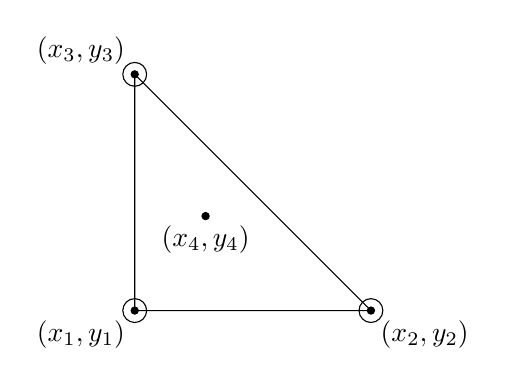
\begin{tikzpicture}
		\draw node[anchor=north east]{$(x_1,y_1)$} (0,0) --  (3,0) node[anchor=north west]{$(x_2,y_2)$} -- (0,3) node[anchor=south east]{$(x_3,y_3)$} -- (0,0);
		\draw[black,fill=black] (0,0) circle (.3ex);
		\draw[black] (0,0) circle (1ex);
		\draw[black,fill=black] (3,0) circle (.3ex);
		\draw[black] (3,0) circle (1ex);
		\draw[black,fill=black] (0,3) circle (.3ex);
		\draw[black] (0,3) circle (1ex);
		\draw[black,fill=black] (.9,1.2) circle (.3ex) node[anchor=north]{$(x_4,y_4)$};
	\end{tikzpicture}
\end{frame}
\begin{frame}
\frametitle{Example}

	Let $\{N_1,N_2,...,N_{10}\}$ be a subset of the dual of $P$ defined as follows.
		\linebreak\linebreak
	$N_1(f)=f(x_1,y_1); \;\;\; N_2(f)=f(x_2,y_2); \linebreak N_3(f)=f(x_3,y_3); \;\;\; N_4(f)=f(x_4,y_4); $
	\linebreak\linebreak
	$N_5(f)=\frac{\partial f}{\partial x}(x_1,y_1); \;\;\; N_6(f)=\frac{\partial f}{\partial x}(x_2,y_2); \;\;\; N_7(f)=\frac{\partial f}{\partial x}(x_3,y_3);$
		\linebreak\linebreak
		
	$N_8(f)=\frac{\partial f}{\partial y}(x_1,y_1); \;\;\; N_9(f)=\frac{\partial f}{\partial y}(x_2,y_2); \;\;\; N_{10}(f)=\frac{\partial f}{\partial y}(x_3,y_3);$
		\linebreak\linebreak
	The nodal basis for $P$ is $\{\phi_1,\phi_2,...,\phi_{10}\}$ such that $N_i(\phi_j)=\delta_{ij} \;\;\; \forall i,j \in \{1,2,...,10\}$.
\end{frame}
\begin{frame}
\frametitle{Example}
To find a $\phi_l$ as follows. $$\phi_l(x,y)=a_1 x^3+a_2 x^2 y+a_3 x y^2+a_4 y^3+a_5 x^2+a_6 xy+a_7 y^2+a_8 x+a_9 y+a_{10}$$
	
	We solve the following.
	$$
	\begin{bmatrix}
	x_1^3 & x_1^2 y_1& x_1 y_1^2& y_1^3& x_1^2& x_1y_1& y_1^2& x_1& y_1& 1\\[0.15cm]
	x_2^3 & x_2^2 y_2& x_2 y_2^2& y_2^3& x_2^2& x_2y_2& y_2^2& x_2& y_2& 1\\[0.15cm]
	x_3^3 & x_3^2 y_3& x_3 y_3^2& y_3^3& x_3^2& x_3y_3& y_3^2& x_3& y_3& 1\\[0.15cm]
	x_4^3 & x_4^2 y_4& x_4 y_4^2& y_4^3& x_4^2& x_4y_4& y_4^2& x_4& y_4& 1\\[0.15cm]
	
	3x_1^2 & 2x_1y_1 & y_1^2& 0& 2x_1& y_1& 0& 1& 0& 0\\[0.15cm]
	3x_2^2 & 2x_2y_2 & y_2^2& 0& 2x_2& y_2& 0& 1& 0& 0\\[0.15cm]
	3x_3^2 & 2x_3y_3 & y_3^2& 0& 2x_3& y_3& 0& 1& 0& 0\\[0.15cm]
	
	0 & x_1^2 & 2x_1 y_1& 3y_1^2& 0& x_1& 2y_1& 0& 1& 0\\[0.15cm]
	0 & x_2^2 & 2x_2 y_2& 3y_2^2& 0& x_2& 2y_2& 0& 1& 0\\[0.15cm]
	0 & x_3^2 & 2x_3 y_3& 3y_3^2& 0& x_3& 2y_3& 0& 1& 0\\[0.15cm]
	\end{bmatrix}
	\begin{bmatrix} a_1\\[0.15cm]a_2\\[0.15cm]a_3\\[0.15cm]a_4\\[0.15cm]a_5\\[0.15cm]a_6\\[0.15cm]a_7\\[0.15cm]a_8\\[0.15cm]a_9\\[0.15cm]a_{10} \end{bmatrix}
	=\begin{bmatrix} 0 \\[.15cm]0\\[.15cm]0\\[.15cm]1 \\[.15cm]0\\[.15cm]0\\[.15cm]0\\[.15cm]0\\[.15cm]0\\[.15cm]0 \end{bmatrix}
	$$
\end{frame}
\begin{frame}
\frametitle{Example}
The square matrix $M$ is same for all $\phi_l$.
	So we need to calculate the inverse of $M$ only once. After that, we can get the coefficients of the polynomial $\phi_l$ by taking the $l^{th}$ column of the inverse matrix.
	$$
	[a_i]_{10\times 1}=M^{-1} [\delta_{il}]_{10\times 1}=\mbox{ the }l^{th}\mbox{ column of }M^{-1}
	$$
\end{frame}
\begin{frame}[fragile]
\frametitle{Example}
Program for finding $M$:

	\begin{lstlisting}
	for i in {1,...,10}
	.	(x,y) = location(N_i)
	.	j = 0
	.	for d in {0,...,3}:
	.	.	for px in {0,...,d}:
	.	.	.	if i <= 4
	.	.	.	.	M(i,10-j) = x^(px) * y^(d-px)
	.	.	.	else if i <= 7
	.	.	.	.	if px == 0
	.	.	.	.	.	M(i,10-j) = 0
	.	.	.	.	else
	.	.	.	.	.	M(i,10-j) = px * x^(px-1) * y^(d-px)
	.	.	.	else
	.	.	.	.	if d-px == 0
	.	.	.	.	.	M(i,10-j) = 0
	.	.	.	.	else
	.	.	.	.	.	M(i,10-j) = (d-px) * x^(px) * y^(d-px-1)
	.	.	.	j = j+1
\end{lstlisting}
	
\end{frame}
\begin{frame}
\frametitle{Example}
For an illustration, if $(x_1,y_1)=(0,0)$, $(x_2,y_2)=(1,0)$, $(x_3,y_3)=(0,1)$, $(x_4,y_4)=(0.3,0.4)$, we get the following matrix $M$.
	$$
	\begin{bmatrix}
	0 & 0 & 0 & 0 & 0 & 0 & 0 & 0 & 0 & 1 \\
	1 & 0 & 0 & 0 & 1 & 0 & 0 & 1 & 0 & 1 \\
	0 & 0 & 0 & 1 & 0 & 0 & 1 & 0 & 1 & 1 \\
	0.027 & 0.036 & 0.048 & 0.064 & 0.09 & 0.12 & 0.16 & 0.3 & 0.4 & 1.0 \\
	0 & 0 & 0 & 0 & 0 & 0 & 0 & 0 & 0 & 1 \\
	3 & 0 & 0 & 0 & 2 & 0 & 0 & 1 & 0 & 0  \\
	0 & 0 & 1 & 0 & 0 & 1 & 0 & 1 & 0 & 0  \\
	0 & 0 & 0 & 0 & 0 & 0 & 0 & 1 & 0 & 0  \\
	0 & 1 & 0 & 0 & 0 & 1 & 0 & 0 & 1 & 0  \\
	0 & 0 & 0 & 3 & 0 & 0 & 2 & 0 & 1 & 0  \\
	\end{bmatrix}
	$$
	
\end{frame}

\begin{frame}
\frametitle{Numerical Integration}
After knowing the coefficients, the integration of polynomial functions can be computed exactly using symbolic integration or pre-calculated quadrature rules.
\linebreak\linebreak
For any specified $k$, quadrature rules can be calculated for triangles\footfullcite{dunavant}. Other polygons can be divided into triangles.
\linebreak\linebreak
For non-polynomial functions, there is no method in general to compute the exact integral.
\end{frame}


\begin{frame}
\frametitle{Convergence}
For $\Omega=[0,1]\times[0,1]$, $f\equiv 4$ and $\Gamma=\{0,1\}\times[0,1]$, we get the following convergence in $L^{\infty}$.
\linebreak\linebreak
\begin{tabular}{|c|c|}
\hline
$h$ & Error($\Delta$)  	\\ \hline
1/2	&		0.05555555555555747	 \\ \hline
1/4	&		0.012254901960786158 \\ \hline
1/6	&		0.0054246165357296205 \\ \hline
1/8	&		0.0030509820912780483 \\ \hline
1/10	&		0.0019526216671635899 \\ \hline
1/12	&		0.0013559871283986558 \\ \hline
1/14	&		0.0009962354382344885 \\ \hline
1/16	&		0.0007627427573298484 \\ \hline
1/18	&		0.0006026609440618474 \\ \hline
1/20	&		0.00048815536469060117 \\ \hline
\end{tabular}


%\begin{tabular}{|c|c|c|}
%\hline
%h$ & Error($\Delta$) & $\frac{\Delta}{h^2 log(1/h)}$ 	\\ \hline
%1/2	&		0.05555555555555747	& 0.738206243308329 \\ \hline
%1/4	&		0.012254901960786158	& 0.325679224989007 \\ \hline
%1/6	&		0.0054246165357296205	& 0.250961744506594 \\ \hline
%1/8	&		0.0030509820912780483	& 0.216216386688315 \\ \hline
%1/10	&		0.0019526216671635899	& 0.195262166716359 \\ \hline
%1/12	&		0.0013559871283986558	& 0.180935451949829 \\ \hline
%1/14	&		0.0009962354382344885	& 0.170366782606806 \\ \hline
%1/16	&		0.0007627427573298484	& 0.162161702063736 \\ \hline
%1/18	&		0.0006026609440618474	& 0.155553591018843 \\ \hline
%1/20	&		0.00048815536469060117	& 0.150082739465656 \\ \hline
%\end{tabular}

\end{frame}


\frame{
{Plot}
Solution plot for $h=1/8$.
\linebreak
\linebreak
\includegraphics[width=200pt]{image1.png}
}


\frame{
{Plot}
Solution plot for $\Gamma=\{0\}\times[0,1]$, $f\equiv 4$, $u(x,y)=y$ on $\Gamma$ and $\frac{\partial u }{ \partial n} = -1$ on $\partial \Omega-\Gamma$.
\linebreak
\linebreak
\includegraphics[width=200pt]{image2.png}
}


\begin{frame}
\frametitle{Mesh refinement}
Based on an error indicator, e.g., the Eriksson-Johnson error indicator, mesh refinement is done selectively for computational efficiency and this leads to faster convergence in same computational effort\footfullcite{gockenbach}.
\linebreak\linebreak
For example, for discretisation with piecewise linear functions, an estimate of the second derivative is a good indicator of relative error.
\end{frame}




\begin{frame}
\frametitle{Mesh refinement}
Example mesh refinement in conforming FEM using the Newest-node bisection algorithm.
\linebreak
\linebreak
		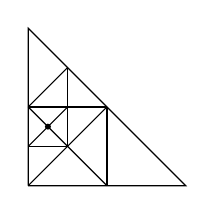
\begin{tikzpicture}
		\draw (0,0) --  (2,0) -- (0,2) --(0,0);\pause
		\draw (0,0) -- (1,1);\pause
		\draw (0,1)--(1,1);\pause
		
		\draw (0,1)--(.5,.5);\pause
		\draw (1,1)--(1,0);	\pause
		\draw (.5,.5)--(1,0);\pause
		
		\draw (.5,.5)--(.5,1);\pause
		\draw (.5,1.5)--(0,1); \pause
		\draw (.5,1)--(.5,1.5);\pause
		
		\draw (.5,1)--(.25,.75);\pause
		\draw (0,.5)--(.5,.5);\pause
		\draw (0,.5)--(.25,.75);
		\draw[black,fill=black] (.25,.75) circle(.2ex);
	\end{tikzpicture}
\end{frame}


\begin{frame}
\frametitle{Mesh refinement}
		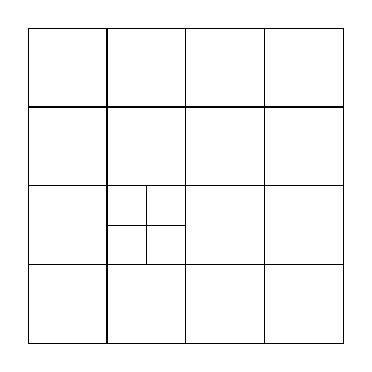
\begin{tikzpicture}
		\draw (0,0)--(4,0)--(4,4)--(0,4)--(0,0);
		\draw (1,0)--(1,4); \draw (2,0)--(2,4); \draw (3,0)--(3,4); 
		\draw (0,1)--(4,1); \draw (0,2)--(4,2); \draw (0,3)--(4,3); 
		\draw (1.5,1)--(1.5,2);
		\draw (1,1.5)--(2,1.5);
	\end{tikzpicture}
	\linebreak
	\linebreak
	In conforming FEM this type of refinement can't be done, though this can be done in non-conforming FEM or the VEM.
	
\end{frame}


\begin{frame}
\frametitle{FEM}
Elements with triangular, quadrilatral or other polygonal shapes have to be studied seperately.
\linebreak\linebreak
If the finite dimensional approximation space $V_h$ contains non-polynomial functions, then the basis functions have to be computed numerically, which, depending on the space, may be a complex problem.
\linebreak After that, $a(v_1,v_2)$ and $(f,v)$ need to be approximated using numerical integration which becomes computationally expensive.
\linebreak\linebreak
When the basis functions are $k$-degree polynomials, we can compute $a(v_1,v_2)$ and $(f,v)$ exactly using, for each element, the inverse of a square matrix with each dimension $(k+1)(k+2)/2$, which has to be computed once for each element. With increasing $k$, the computational complextity increases manyfold.
\end{frame}

\begin{frame}\frametitle{Introduction to VEM\footfullcite{vem}}
Generalizes FEM to arbitrary polygonal mesh.
\linebreak\linebreak
Each element can be a polygon with arbitrary number of sides.
\linebreak\linebreak
Allows computation of the stiffness matrix using the degrees of freedom even though the canonical basis includes non-polygonal functions.
\end{frame}
\begin{frame}
\frametitle{Mesh}
Let $\{T_h\}_h$ be a sequence of decompositions of $\Omega$ into elements $K$ satisfiying the following.
\begin{itemize}
\item Each $K$ is a simple polygon.
\item There exists a $\gamma_1$ such that for all $h$, each $K$ in $T_h$ is star-shaped with respect to a ball of radius greater than $\gamma_1 h_K$.
\item There exists a $\gamma_2$ such that for all $h$, for each $K$ in $T_h$, the distance between any two vertices is greater than $\gamma_2 h_K$
\end{itemize}
\end{frame}
\begin{frame}
\frametitle{Discretization}
Define, for $K\in T_h$,\linebreak $\mathbb{B}_k(\partial K):=\{v\in C^0(\partial K):v_{|e}\in\mathbb{P}_k(e)$ $\forall e \in \partial K\}$.
\linebreak\linebreak
Define, for $K\in T_h$,\linebreak $V^{K,k}:=\{v\in H^1(K) : v_{|\partial K} \in \mathbb{B}_k(\partial K)$ and $ \Delta v_{|K} \in \mathbb{P}_{k-2}(K)\}$.
\linebreak\linebreak
Define $V_h:=\{v\in V : v_{|K}\in V^{K,k}$ $\forall K \in T_h \}$.
\linebreak\linebreak
\noindent\fbox{%
    \parbox{\textwidth}{%
\textbf{Note -} $\mathbb{P}_k(K)\subset V^{K,k}$
}%
}
\end{frame}

\begin{frame}
\frametitle{Degrees of freedom}
We have the following degrees of freedom\footfullcite{vem} for $V_h$.
\begin{itemize}
\item The values of $v_h$ at internal vertices.
\item The values of $v_h$ at $k-1$ uniformly spaced points on each internal edge $e$.
\item For $k>1$, the moments $\frac{1}{|K|}\int_K m(x) v_h(x) dx$ $\forall m \in M_{k-2}(K)$ in each element $K$.
\end{itemize}
Where $\it{M}_{k-2}(K):=\{ \big(\frac{x-x_{K}}{h_{k}}\big)^{s}, |s|\leq k-2 \} $ and $x_{K}$ denotes the barycentre of $K$.
\end{frame}
%\frame{
%\frametitle{Degrees of freedom}

%\noindent\fbox{%
%    \parbox{\textwidth}{%
%\textbf{Remark -} The degrees of freedom choosen have the following properties.
%\begin{itemize}
%\item On each internal edge, the degrees of freedom specify a polynomial of degree $k$.
%\item In the interior of each element, the degrees of freedom specify the $L^2$ projection of the function into the space $\mathbb{P}_{k-2}(K)$. Note that $M_{k-2}(K)$ is a basis of $\mathbb{P}_{k-2}(K)$.
%\end{itemize}
%}%
%}
%}
\begin{frame}
\frametitle{Approximate Bilinear Form}
Define $\Pi_k^K:V^{K,k}\to \mathbb{P}_k(K)$ which takes $v\in V^{K,k}$ to the solution of the following equations.
$$ a^K(\Pi_k^Kv,q)=a^K(v,q)\;\;\forall q \in \mathbb{P}_k(K) $$
$$ j_K(\Pi_k^Kv)=j_K(v) $$
Where $j_K(q)$ denotes the average of $q$ over the vertices of $K$.
\linebreak\linebreak
%Note that for $v\in V^{K,k}$ and $q \in \mathbb{P}_k(K)$, we have following.
%$$a^K(v,q)=\int_K \triangledown v \cdot \triangledown q\;dx = - \int_K  v \Delta q\; dx + \int_{\partial K} \frac{\partial q}{\partial n}v\;ds$$
\end{frame}
\begin{frame}
\frametitle{Approximate Bilinear Form}
Define the bilinear form $S^K$ on $V^{K,k}$ as $ S^K (u,v)=\sum\limits_{r=1}^{N^K} \chi_r (u)\chi_r (v) $.
\linebreak Where $\chi_r$ are the degrees of freedom in $K$.
\linebreak\linebreak
Thus define $a_h^K(u,v)=a^K(\Pi_k^Ku,\Pi_k^Kv)+S^K(u-\Pi_k^Ku,v-\Pi_k^Kv)$.
\end{frame}

\begin{frame}
\frametitle{Properties of the approximate Bilinear Form}
\noindent\fbox{%
    \parbox{\textwidth}{%
\textbf{Remark -} The approximate bilinear form has been constructed such that it satisfies these properties.
\begin{itemize}
\item \textbf{$k$-Consistency -} For all $p \in \mathbb{P}_k(K)$ and for all $v_h \in V_{h|K}$, $a_h^K(p,v_h)=a^K(p,v_h)$.
\item \textbf{Stability -} There exist two positive constants $\alpha_*$ and $\alpha^*$ , independent of $h$ and of $K$, such that for all $v_h \in V_{h|K}$,
$\alpha_* a^K (v_h , v_h ) \le a^K_h (v_h , v_h ) \le \alpha^* a (v_h , v_h )$.
\linebreak\linebreak
We needed the property that vertices are not arbitrarily close to each other for this.
\end{itemize}
}%
}
\end{frame}

\begin{frame}
\frametitle{Approximation of the load function}
For $k\ge 2$, define $F_h v=\sum\limits_{K\in T_h}\int_K(P_{k-2}^K f)v\;dx=\sum\limits_{K\in T_h}\int_K f(P_{k-2}^K v)\;dx$.
\linebreak
Where $P_{k-2}^K f$ is the $L^2$ projection of $f$ in $\mathbb{P}_{k-2}(K)$.
\linebreak\linebreak
For $k=1$, define $F_h v=\sum\limits_{K\in T_h}\int_K(P_0^K f)j_K(v)\;dx$
\linebreak\linebreak
Let $b_h$ be the smallest constant such that $(f,v)-F_hv\le b_h |v|_1\;\forall v \in V_h$.
\linebreak
Then we have the follwing bound.
$$b_h\le Ch\sqrt{\sum\limits_{K\in T_h}|f|_{min(1,k-1),K}^2}$$
\end{frame}

\begin{frame}
\frametitle{Error Estimates}
\textbf{Theorem} Let $u_h$ be the solution of $a_h(u_h,v_h)=F_h v\;\forall v \in V_h$. Then we have the following for all $u_I\in V_h$ and $u_{\pi}$ piecewise in $\mathbb{P}_k$.
$$
|u-u_h|_1\le C(|u-u_I|_1 + |u-u_{\pi}|_{h,1} + b_h)
$$
Where $|v|_{h,1}=\sqrt{\sum\limits_{K\in T_h}|\triangledown v|_{0,K}^2}$.
\end{frame}

\begin{frame}
\frametitle{Interpolation and Projection Errors}
We have the following\footfullcite{brenner}.\linebreak\linebreak
There exists $C$ such that for all $s\in[2,k+1]$, for all $h$, for all $K\in T_h$, for all $w \in H^s(K)$, there exists a $w_I \in V^{K,k}$ such that following holds.
$$||w-w_I||_{0,K}+h_K|w-w_I|_{1,K}\le C h_K^s |w|_{s,K}$$
\linebreak\linebreak
There exists $C$ such that for all $s\in[2,k+1]$, for all $h$, for all $K\in T_h$, for all $w \in H^s(K)$, there exists a $w_{\pi} \in \mathbb{P}_k(K)$ such that following holds.
$$||w-w_{\pi}||_{0,K}+h_K|w-w_{\pi}|_{1,K}\le C h_K^s |w|_{s,K}$$
\end{frame}

\frame{
\frametitle{Proof of Theorem}
As $a(.,.)$ is continuous and elliptic, and $a_h(.,.)$ satisfies the stability property, i.e., $\alpha_* a^K (v_h , v_h ) \le a^K_h (v_h , v_h ) \le \alpha^* a (v_h , v_h )$ for all $v_h \in V_h$, $a_h(.,.)$ is continuous and also an inner product on $V_h$.
\linebreak
Thus, $a_h(u,v)\le \sqrt{a_h(u,u)a_h(v,v)}\le \alpha^*\sqrt{a(u,u)a(v,v))} \le \alpha^* M |u||v|$.
Thus, $a_h(.,.)$ is elliptic, hence we get the existence and uniquness of the solution.
\linebreak\linebreak
Next, we prove the inequality.
}

\frame{
\frametitle{Proof of Theorem}
Let $\delta_h=u_h-u_I$.
\begin{equation*}
\begin{split}
\alpha_*|\delta_h|^2_1 & =  \alpha_*a(\delta_h,\delta_h)\le a_h(\delta_h,\delta_h) \\
& =a_h(u_h,\delta_h)-a_h(u_I,\delta_h) \\
& =F_h\delta_h-\sum\limits_K a_h^K(u_I,\delta_h) \\
& =F_h\delta_h-\sum\limits_K (a_h^K(u_I-u_{\pi},\delta_h)+a_h^K(u_{\pi},\delta_h)) \\
& =F_h\delta_h-\sum\limits_K (a_h^K(u_I-u_{\pi},\delta_h)+a^K(u_{\pi},\delta_h)) \\
& =F_h\delta_h-\sum\limits_K (a_h^K(u_I-u_{\pi},\delta_h)+a^K(u_{\pi}-u,\delta_h))-a(u,\delta_h) \\
& =F_h\delta_h-\sum\limits_K (a_h^K(u_I-u_{\pi},\delta_h)+a^K(u_{\pi}-u,\delta_h))-(f,\delta_h) \\
& =F_h\delta_h-(f,\delta_h) -\sum\limits_K (a_h^K(u_I-u_{\pi},\delta_h)+a^K(u_{\pi}-u,\delta_h)) \\
\end{split}
\end{equation*}
}



\frame{
\frametitle{Proof of Theorem}
Thus we get $|\delta_h|^2_1\le C_1 (b_h+|u_I-u_{\pi}|_{h,1}+|u-u_{\pi}|_{h,1}) |\delta_h|_1$.\linebreak
Hence, $|u_h-u_I|_1\le C_1 (b_h+|u_I-u_{\pi}|_{h,1}+|u-u_{\pi}|_{h,1})$.\linebreak
Now we get the following. 
\begin{equation*}
\begin{split}
|u-u_h|_1 & \le |u-u_I|_1+|u_I-u_h|_1 \\
& \le |u-u_I|_1+C_1 (b_h+|u_I-u_{\pi}|_{h,1}+|u-u_{\pi}|_{h,1})\\
& \le |u-u_I|_1+C_1 (b_h+|u_I-u|_{h,1}+|u-u_{\pi}|_{h,1}+|u-u_{\pi}|_{h,1})\\
& =C(|u-u_I|_1 + |u-u_{\pi}|_{h,1} + b_h)
\end{split}
\end{equation*}
}

\begin{frame}
\frametitle{Computational Aspects / Stiffness Matrix}
Like in FEM, we compute the contribution of each element to the stiffness matrix seperately.
\linebreak\linebreak
Let $\phi_i$ and $\phi_j$ be two nodal basis functions of $V^{K,k}$. We need to compute $a_h(\phi_i,\phi_j)=a^K(\Pi_k^K\phi_i,\Pi_k^K\phi_j)+S^K(\phi_i-\Pi_k^K\phi_i,\phi_j-\Pi_k^K\phi_j)$.
\linebreak\linebreak
$a^K(\Pi_k^K\phi_i,\Pi_k^K\phi_j)$ can be computed exactly once $\Pi_k^K\phi_i$ and $\Pi_k^K\phi_j$ are computed as they are polynomials.
\linebreak\linebreak
Computation of $S^K(\phi_i)$ involves computing $\chi_r (\phi_i)$ for $r$ in $\{1,2,...,N^K\}$, which are the degrees of freedom of $\phi_i$ which are known by the definition of $\phi_i$.
\end{frame}

\begin{frame}
\frametitle{Computational Aspects / Projection Operator}
For the projection operator, we need to solve the following set of equations.
$$ a^K(\Pi_k^Kv,q)=a^K(\phi_i,q)\;\;\forall q \in \mathbb{P}_k(K) $$
$$ j_K(\Pi_k^Kv)=j_K(\phi_i) $$
Note that varying $q$ over the basis of $\mathbb{P}_k(K)$ suffices. Thus, a system of linear equations is formed.
\linebreak\linebreak
$j_K(\phi_i)$, the average of $\phi_i$ over the vertices is exactly computable as the degrees of freedom include the value at vertices.
\end{frame}
\begin{frame}
\frametitle{Computational Aspects / Projection Operator}
$a^K(\phi_i,q)=\int\limits_{K}\triangledown \phi_i \cdot \triangledown q \;dx$.
\linebreak
Applying Green's theorem, this is equal to $\int\limits_{K} \Delta q \phi_i\;dx + \int\limits_{\partial K}\frac{\partial q}{\partial n} \phi_i\;ds$.
\linebreak\linebreak
The first term can be computed exactly because $\Delta q$ is in ${P}_{k-2}(K)$ and the degrees of freedom involve the moments $\frac{1}{|K|}\int_K m(x) \phi_i(x) dx$ for all $m$ in $ M_{k-2}(K)$ which is a basis of ${P}_{k-2}(K)$.
\linebreak\linebreak
The second term is also computable as the integrand is a polynomial on $\partial K$.
\end{frame}

\frame
{
	\frametitle{Mixed Methods\footfullcite{gabriel}}
	We have two real Hilbert spaces $H$ and $Q$ and two continuous bilnear forms $a:H\times H\to\R$ and $b:H\times Q \to \R$. We are given $F\in H'$ and $G\in Q'$ and have to find $(\sigma,u)\in H\times Q$ satisfiying the following.

\begin{equation*}
\begin{split}
a(\sigma . \tau)+b(\tau , u) & = F(\tau) \;\; \forall \tau \in H \\
b(\tau,v) & =G(v) \;\; \forall v \in Q \\
\end{split}
\end{equation*}
The ellipticity of $a(.,.)$ and the inf-sup condition on $b(.,.)$ are sufficient for the existence and uniquness of the solution of the above equations.
\begin{equation*}
\inf\limits_{v\in Q-\{0\}} \sup\limits_{\tau\in H-\{0\}} \frac{b(\tau,v)}{||\tau||_H||v||_Q} \ge \beta
\end{equation*}
}

\frame
{
	\frametitle{Mixed Methods}
We take two subspaces $H_h$ and $Q_h$ of $H$ and $Q$ respectively such that the Inf-Sup condition for $b(.,.)$ is satisfied.
\begin{equation*}
\inf\limits_{v\in Q_h-\{0\}} \sup\limits_{\tau\in H_h-\{0\}} \frac{b(\tau,v)}{||\tau||_H||v||_Q} \ge \beta
\end{equation*}
Then solve these equations.
\begin{equation*}
\begin{split}
a(\sigma . \tau)+b(\tau , u) & = F(\tau) \;\; \forall \tau \in H_h \\
b(\tau,v) & =G(v) \;\; \forall v \in Q_h \\
\end{split}
\end{equation*}
For example, Raviart-Thomas spaces of order $k=1$ can be used here. For two dimensional domain, they are the functions $\{(p_1(x_1,x_2)+p_0(x_1,x_2)x_1,p_2(x_1,x_2)+p_0(x_1,x_2)x2)$\linebreak for $p_0,p_1,p_2\in \mathbb{P}_k(\Omega)\}$.
}

%\frame
%{
%	\frametitle{TODO}
%	We plan to work on the Mixed Virtual Element Method\footfullcite{mvem}, more specifically on creating stabilizer for MVEM.
%	\linebreak\linebreak
%	Stabilizers, for one, allow to circumvent the Inf-Sup condition, which permits the use of independent discretisation of different unknowns, e.g. pressure %and velocity in the fluid flow problem.
%}
\frame
{
	{Future plan}
\begin{itemize}
\item Implementation of conforming VEM for elliptic problems.
\item To carry out a detailed study of  mixed FEM for elliptic, Stokes problem with an emphasis on inf-sup condition.
\item To study mixed and non conforming VEM for elliptic and parabolic problems.
\item Implementation of mixed and nonconforming VEM for elliptic and Stokes problems.
\item  To develop stabilized mixed  VEM ( Need to add a stabilizer when inf-sup is not satisfied by discrete spaces). These methods are not very well developed in the literature.   
\end{itemize}
}


\frame{
\frametitle{References}
\nocite{pani}
\nocite{ciarlet}
\nocite{mvem}
\printbibliography
}
\end{document}
